\documentclass[12pt]{article}\usepackage[]{graphicx}\usepackage[]{color}
%% maxwidth is the original width if it is less than linewidth
%% otherwise use linewidth (to make sure the graphics do not exceed the margin)
\makeatletter
\def\maxwidth{ %
  \ifdim\Gin@nat@width>\linewidth
    \linewidth
  \else
    \Gin@nat@width
  \fi
}
\makeatother

\definecolor{fgcolor}{rgb}{0.345, 0.345, 0.345}
\newcommand{\hlnum}[1]{\textcolor[rgb]{0.686,0.059,0.569}{#1}}%
\newcommand{\hlstr}[1]{\textcolor[rgb]{0.192,0.494,0.8}{#1}}%
\newcommand{\hlcom}[1]{\textcolor[rgb]{0.678,0.584,0.686}{\textit{#1}}}%
\newcommand{\hlopt}[1]{\textcolor[rgb]{0,0,0}{#1}}%
\newcommand{\hlstd}[1]{\textcolor[rgb]{0.345,0.345,0.345}{#1}}%
\newcommand{\hlkwa}[1]{\textcolor[rgb]{0.161,0.373,0.58}{\textbf{#1}}}%
\newcommand{\hlkwb}[1]{\textcolor[rgb]{0.69,0.353,0.396}{#1}}%
\newcommand{\hlkwc}[1]{\textcolor[rgb]{0.333,0.667,0.333}{#1}}%
\newcommand{\hlkwd}[1]{\textcolor[rgb]{0.737,0.353,0.396}{\textbf{#1}}}%
\let\hlipl\hlkwb

\usepackage{framed}
\makeatletter
\newenvironment{kframe}{%
 \def\at@end@of@kframe{}%
 \ifinner\ifhmode%
  \def\at@end@of@kframe{\end{minipage}}%
  \begin{minipage}{\columnwidth}%
 \fi\fi%
 \def\FrameCommand##1{\hskip\@totalleftmargin \hskip-\fboxsep
 \colorbox{shadecolor}{##1}\hskip-\fboxsep
     % There is no \\@totalrightmargin, so:
     \hskip-\linewidth \hskip-\@totalleftmargin \hskip\columnwidth}%
 \MakeFramed {\advance\hsize-\width
   \@totalleftmargin\z@ \linewidth\hsize
   \@setminipage}}%
 {\par\unskip\endMakeFramed%
 \at@end@of@kframe}
\makeatother

\definecolor{shadecolor}{rgb}{.97, .97, .97}
\definecolor{messagecolor}{rgb}{0, 0, 0}
\definecolor{warningcolor}{rgb}{1, 0, 1}
\definecolor{errorcolor}{rgb}{1, 0, 0}
\newenvironment{knitrout}{}{} % an empty environment to be redefined in TeX

\usepackage{alltt}

%\usepackage{endfloat}
% \usepackage{type1ec}
% \usepackage{subcaption}
% \usepackage{fullpage}
% \usepackage{enumerate}
% \usepackage{graphicx}
% \usepackage{graphics}
% \usepackage{multirow}
\usepackage{comment}
\usepackage{amsmath,amssymb,amsfonts,amsthm}
\usepackage{setspace}
%\usepackage{verbatim}
\usepackage{natbib}
\usepackage{bm}
\usepackage{pdflscape}
%\usepackage{tikz}
%\usepackage{xr}
\usepackage[colorlinks=true,linkcolor=green]{hyperref}

\newcommand{\dalphaU}{\bar{d}_\alpha}
\newcommand{\dalphaB}{\underline{d}_\alpha}
\newcommand{\dstar}{d^*}
\newcommand{\ps}{\bm{p}_D}
\newcommand{\dhat}{\hat{d}}
\newcommand{\dhatU}{\bar{d}}
\newcommand{\dhatB}{\underline{d}}
\newcommand{\dhatm}{\hat{d}_M}
\newcommand{\dhatmab}{\hat{d}^{ab}_M}
\newcommand{\EE}{\mathbb{E}}

\newcommand\independent{\protect\mathpalette{\protect\independenT}{\perp}}
\def\independenT#1#2{\mathrel{\rlap{$#1#2$}\mkern2mu{#1#2}}}


\doublespacing

\def\independenT#1#2{\mathrel{\rlap{$#1#2$}\mkern2mu{#1#2}}}
\newtheorem{conjecture}{Conjecture}
\newtheorem{ce}{Counter-Example}
%\newtheorem{ass}{Assumption}
\newtheorem{alg}{Algorithm}
%\newtheorem*{ass*}{Assumption}
\newtheorem{prop}{Proposition}
\newtheorem{lemma}{Lemma}
\newtheorem{remark}{Remark}

\newenvironment{ass}[2][Assumption:]{\begin{trivlist}
\item[\hskip \labelsep {\bfseries #1}\hskip \labelsep {\bfseries
    #2}.]}{\end{trivlist}}

\defcitealias{bls}{BLS}









\title{Sequential Specification Tests to Choose a Model: A
  Change-Point Approach}

\author{Adam Sales}
\IfFileExists{upquote.sty}{\usepackage{upquote}}{}
\begin{document}

\maketitle

\section{Introduction}

One of many mis-matches between best practices recommended by
statisticians and practice in quantitative research regards model
selection.
Statisticians conceptualize model selection as a tradeoff between bias
and variance.
Many quantitative researchers adopt a different outlook, thinking about model selection as choosing
the best model that satisfies the assumptions of their intended
statistical test or estimator---essentially minimizing variance while
constraining bias at zero.
This latter outlook leads researchers towards hypothesis tests of
model assumptions; in particular, ``sequential specification tests'' (SSTs): a sequence of hypothesis tests, for
a sequence of models, ordered by preferability.
The best model whose assumptions ``pass'' a hypothesis test is chosen.

Do hypothesis tests make any sense in model selection?
For one, ``all models are wrong''
\citep[p. 2]{modelsWrong} and ``there's no such thing as unbiased
estimation'' \citep{gelmanBlogUnbiased}, so the search for a correct
model might be hopeless, and therefore pointless.
Further, the logic of null-hypothesis testing seems incompatible
with this framework.
The results of a null hypothesis test, of course, are never evidence
in favor of a null hypothesis---null hypotheses can only be rejected,
not accepted.

On the other hand, ``some models are useful,'' and depending on their
intended use, their usefulness may depend on \emph{approximate}
correctness.
If so, hypothesis tests may have a role to play.
Specification tests already exist for most common models, and
they are regularly taught in introductory quantitative methods
classes.
If their use in model selection could be made conceptually sound, they
are likely to be actually used---and maybe even correctly.

This paper will apply a clever idea from change-point or threshold
estimation to the more general problem of model selection from SSTs.
\citet{mallik} points out that in a process with a change point,
the p-values from a sequence of tests of a null regression function
are uniformly-distributed as long as the regression function is
correct, but asymptotically zero when the function is not correct.
They use this dichotomous behavior to construct a simple, consistent
estimator of the change-point---the point at which the null model
stops being correct.

In the same way, their estimator can choose the change-point in
a sequence of models, when models stop being correct.
In doing so, it shifts the model selection rationale away
from the logic of hypothesis testing and towards the logic of
estimation.
In the tradition of constructing confidence intervals from hypothesis
tests and \citet{hodgeslehmann}, their estimator exploits
the behavior of hypothesis tests to estimate quantities of interest.
Further, as opposed to model selectors based on strict
hypothesis-testing logic, an individual test result will itself not
drive the change-point estimator, which is instead based on the entire
sequence of p-values.
Thus, the change-point view of model selection is arguably conceptually
more satisfying and practically more reliable than the conventional
test-based approach.
What's more, unlike other SST model selectors, the change-point
approach does not require the researcher to specify a level $\alpha$
or any other tuning parameter.

The following sub-section will briefly introduce two running examples
of sequential specification tests: choosing a bandwidth for a
regression discontinuity design and choosing a lag order for a
time-series model.
Next, section \ref{sec:setup} will review the formalism of SSTs and
discuss common SST-based model selectors.
Section \ref{sec:change-point} will introduce the new method, section
\ref{sec:simulation} will demonstrate some of its properties in a
simulation study, \ref{sec:examples} will apply it to the running
examples, and \ref{sec:discussion} will conclude.

\subsection{SSTs in Regression Discontinuity and Time Series}\label{sec:exampleIntro}

\begin{figure}

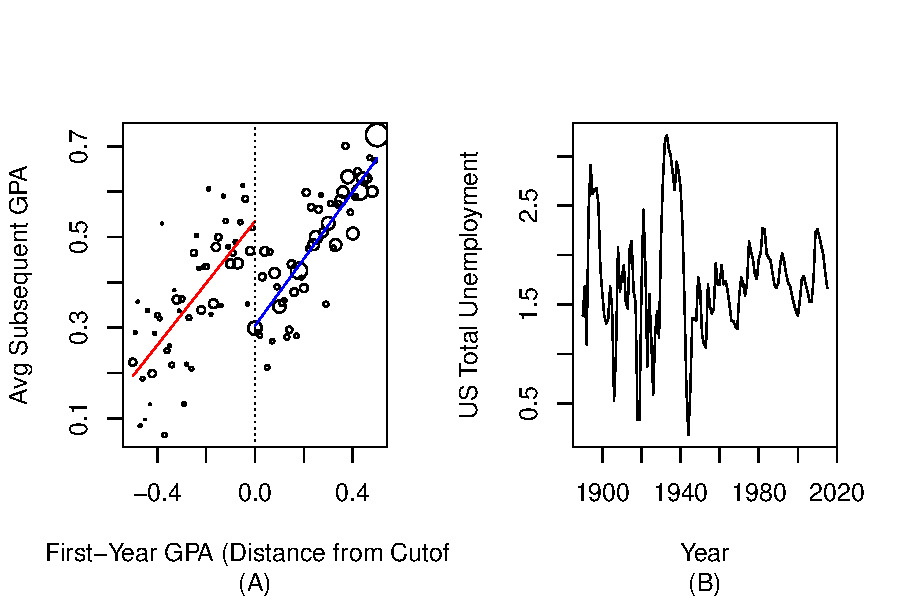
\includegraphics[width=\maxwidth]{figure/examplePlots-1} 

\caption{Two data examples for SSTs. Plot (A) shows data from
  \citet{lso}---subsequent grade point averages (GPAs) for students
  at a large Canadian university, as a function of first-year
  GPAs. Subsequent GPAs are averaged by first-year GPAs, which are
  centered at the academic probation cutoff (dotted line), and the sizes
  of the plotted points are proportional to the number of students
  with each first-year GPA. The red and blue lines are linear least-squares
  fits on either side of the cutoff. Students with first-year GPAs
  to the left of  the cutoff are put on probation. Plot (B) shows a
  time-series of log annual United States total unemployment from 1890 to
  2015. Data were combined from \citet{urca} and \citet{cps}.}
\label{fig:example}
\end{figure}
%%% NOTE: schotman & van dijk used AR(4) for unemployment


Figure \ref{fig:example} displays two datasets that will serve as
illustrations of SSTs.
Section \ref{sec:examples} will discuss both of these examples in more
detail.
The brief overview here will be helpful to fix ideas.

Figure \ref{fig:example}A plots data that \citet{lso} used to estimate the effect of academic
probation.
Students at an unnamed large Canadian University were put on academic
probation---simultaneously given extra help and threatened with
suspension---if their first-year cumulative grade point averages
(GPAs) fell below a cutoff.
This is an example of a regression discontinuity design (RDD) \citep{thistlewhiteCampbell}, in
which treatment (in this case academic probation) is assigned if a
numeric ``running variable'' $R$ (first-year GPA) falls below (or above) a
pre-specified cutoff $c$.
Typically \citep[e.g.][]{imbensLemiuxRDD,angristLavy,lee} analysts
will fit regression models $Y=f_1(R)+\epsilon$ and $Y=f_2(R)+\epsilon$
to data on either side of the cutoff, modeling the relationship
between $R$ and an outcome of interest $Y$.
The difference between the models' predictions when $R$ is set equal
to the $c$ is interpreted as a ``local
average treatment effect,'' roughly speaking the treatment effect when
the running variable is equal to the cutoff \citep{HTV}.
Figure \ref{fig:example}A shows one of the outcomes \citet{lso} considered,
students' subsequent GPAs, along with linear regression models below
(in red) and above (blue) $c$, which is signified with a dotted
line.
A simpler alternative approach, suggested in \citet{cft}, models the
relationships between $Y$ and $R$ on either side of $c$ as constant,
and treats the data as if they were generated by a randomized
experiment.

Of course, misspecified regression models will lead to biased
treatment effect estimators.
To minimize the influence of model misspecification, researchers will
typically fit the regression models using only subjects for whom $R\in
\mathcal{W}_b\equiv (c-b,c+b)$ for some bandwidth $b>0$.
A number of options exist for choosing the RDD bandwidth, including
cross-validation \citep{ludwigMiller} and asymptotic minimization of
mean-squared-error \citep{IK}.
\citet{cft} and others \citet{salesHansen,angristWanna} suggest SSTs
of covariate balance---at a sequence of candidate bandwidths $b$, test
for the presence of a ``treatment effect'' on a pre-treatment
covariate $X$, referred to as covariate imbalance.
A window choice $\mathcal{W}_b$ that, paradoxically, leads to a
statistically significant
treatment effect on a covariate is unacceptable; on the other
hand, larger windows include larger data samples, yielding higher
precision.
Therefore, SSTs could be used to choose the largest $b$ for which a
hypothesis test fails to reject the hypothesis of covariate balance.

Figure \ref{fig:example}B shows the annual total unemployment rate in the
United States from 1890 to 2015.
One of the simpler models for time series such as these is an order
$p$ autoregression, or $AR(p)$ under which the value of the time
series at point $t$ may depend on its historical values at
$t-1,...,t-p$ but, conditional on those, is independent of values at
points before $t-p$.
SSTs can be useful here, too: researchers may test model fit for a
sequence of lag orders $p$, and choose the smallest $p$ that the tests
fail to reject.
Here a smaller lag orders $p$ are preferable since they lead to more
parsimonious models and more precise estimates.



\section{The Setup, in General}\label{sec:setup}

Say, in specifying a model, a researcher must choose from a discrete,
ordered, set of specifications $d=1,2,\dots,D$.
The resulting model must satisfy testable assumption $\mathcal{A}$.
Assume that either $\mathcal{A}$ is false for all $d$, or that for
some $1\le \dstar\le D$, $\mathcal{A}$ is true for $d\le \dstar$ and false
for all $d>\dstar$.
Further assume that if $\dstar$ exists, it is the optimal choice---for
instance, the smallest model, or the biggest dataset, that satisfies
$\mathcal{A}$.
Finally, assume the researcher has chosen a valid, unbiased test of
$\mathcal{A}$ and calculated p-values for each $d$:
$\bm{p}_D=p_1,\dots,p_d,\dots,p_D$.
The procedure here is to use $\bm{p}_D$ to choose a specification
$\hat{d}$ that is as large as possible without violating
$\mathcal{A}$.


A common choice for $d$ in this scenario relies on the logic of null
hypothesis testing: for a pre-specified $\alpha \in (0,1)$, let
\begin{equation*}
\dalphaU \equiv max\{d : p_d>\alpha\}.
\end{equation*}
That is, $\dalphaU$ is the largest value of $d$ for which the
null hypothesis that $\mathcal{A}$ is true for $d\le \dalphaU$
cannot be rejected at level $\alpha$.
Although it may seem as though the multiplicity of tests involved in
this procedure invalidates the null hypothesis framework, it turns out
that this is not the case: the ``stepwise intersection-union
principle'' \citet{berger1988, rosenbaum2008,hansen2015} insures that the
family-wise error rate is maintained.
That is, the probability of falsely rejecting the null---choosing
$\dalphaU<\dstar$, is bounded by $\alpha$.
$\dalphaU$ is the specification that would result from testing null
hypotheses backwards: for $d'=D,D-1,\dots,d,\dots,1$, test $H_{0d'}:$
$\mathcal{A}$ is true for $d\le d'$.
Then, stop testing at $d'=\dalphaU -1$---the first $d'$ for which
$p_{d'} \ge \alpha$; reject all null hypotheses $H_{0d'}$ for which
$d'\ge \dalphaU$, and fail to reject the rest.
This protects the family-wise error rate of $\alpha$ since rejecting
\emph{any} true null implies rejecting the first true null---a
probability $\alpha$ event.

Another common choice for $\hat{d}$  \citep[e.g.][]{lutkepohl2005new}, say $\dalphaB$,
does not have this property.
Let
\begin{equation}
\dalphaB\equiv min\{d: p_d<\alpha\}-1
\end{equation}
$\dalphaB$ selects $\hat{d}$ to be the largest value of $d$ before the first
significant p-value.
This is equivalent to the opposite procedure as $\dalphaU$: start with the $d'=1$
and test sequentially for larger values of $d'$ until the first
rejection, at $\dalphaB$, then stop; reject all null
hypotheses $H_{0d'}$ for $d'\ge \dalphaB$ and fail to
reject the rest.
This procedure does not control family-wise error rates---it is likely
to reject more than $100\alpha$\% valid specifications.

\begin{comment}
This paper will focus on two data scenarios for SSTs, corresponding to
the two examples in Section \ref{sec:exampleIntro}.
In the first, the SSTs help determine which data are included in the
analysis.
For instance, choosing the bandwidth of a regression discontinuity
design, or choosing the parameters of a matching design.
In this scenario, each choice $d$ corresponds to rows in the dataset
that could be included in the analysis.
Formally, let $\mathcal{I}=\{1,\dots,N\}$, indices for $N$ candidate
cases to be fit in a model.
Then let $\mathcal{I}=\mathcal{i}_1\cup\mathcal{i}_2\cup\dots\cup
\mathcal{i}_d \cup \dots union \mathcal{i}_D$.
The choice of $\hat{d}$ means fitting the model to the dataset
including each of these subsets,
$\mathcal{I}_d=\mathcal{i}_1\cup\dots\mathcal{i}_d$.
Note that the sets denoted with lower-case $\mathcal{i}_d$ are disjoint,
$\mathcal{i}_d \cap \mathcal{i}_{d'}=\emptyset$,
those denoted with upper-case $\mathcal{I}_d$ are nested---$d>d'$
implies $\mathcal{I}_{d'}\subset \mathcal{I}_d$, and the full set of
indices, noted without a subscript, $\mathcal{I}=\mathcal{I}_D$.
Finally, let $n_d=|\mathcal{i}_d|$, where $|\cdot |$ denotes
cardinality, and $\bar{n_d}=|\mathcal{I}_d |$.

A second scenario applies when the dataset is fixed, but the model is
not.
Here, $d$ indexes a \emph{pre-specified} sequence of models.
For instance, using SSTs to choose the lag order $p$ in an $AR(p)$
time series model.
Then let $\bm{X}$ denote the full set of variables, $\bm{x}_d$ denote
the set of variables that would be \emph{subtracted} in the $d^{th}$ step
of the sequence, and $\bm{X}_d=\bm{x}_{d+1} \cup \dots \cup \bm{x}_D$
denote the set of variables that would be included in the analysis,
were the analyst to choose $d$.
Note here that bigger values of $d$ correspond to smaller models.
In this scenario, the sample size is fixed at $N$.

\end{comment}

\subsection{Model Selection and the Logic of Null Hypothesis Testing}
In order to avoid certain methodological mistakes, it may be helpful to
clarify some of the conceptual distinctions between SSTs and
conventional null hypothesis tests (NHTs).
The logic of NHTs is familiar to anyone who has taken (and understood)
even the most basic college statistics course; nonetheless we restate
it here to distinguish it from the logic of SSTs.
Typically, researchers use NHTs to reject a null hypothesis that they
consider uninteresting---most of the time, that a model parameter is
equal to zero---and interpret rejection as evidence in favor of an
interesting alternative hypothesis.
NHTs cap the probability of a type-I error---falsely rejecting a true
null hypothesis---and, given that constraint, seek to minimize the
probability of a type-II error, failing to reject a false null
hypothesis.

SSTs reverse some of these elements; most importantly, the goal of
SSTs is to identify specifications in which an assumption
$\mathcal{A}$ is plausible, rather than to identify true alternative
hypothesis.
In the same vein, type-II errors are typically of more concern for
SSTs than for typical NHTs, and type-I errors are less problematic.
In fact, a type-II error from a specification test could lead a
researcher to fit a misspecified model, which in turn may inflate the
probability of a type-I error in her final outcome analysis.
For that reason, some methodologists recommend setting $\alpha$
substantially higher for specification tests than for NHTs in outcome
analyses.
Still, the hypothesis testing framework, in the case of point null
hypotheses, does not allow a researcher to
fix the type-II error rate at a pre-specified value, and then optimize
the type-I error rate, though that might be ideal for
specification tests.

In fact, in continuous data models with continuous parameter spaces,
no hypothesis test can provide any evidence in favor of a point null
hypothesis.
For instance, take the common $H_0: \theta=0$, for some parameter
$\theta\in \mathbb{R}$.
In finite samples, for any type-I or type-II error rate, there will
always be some plausible alternative hypothesis $H_a
\theta=\epsilon\ne 0$.
Further, in these situations, finite sample estimates $\hat{\theta}$
will almost surely be non-zero.
This is important to state to avoid misinterpretations of SST
procedures as providing evidence, or showing, that an assumption
$\mathcal{A}$ is true for certain specifications $d$.
A common Bayesian argument (e.g. \citealp[][p. 439]{kadanePrinciples};
\citealp{gelmanBlog}) states that, theoretically, nearly all null
hypotheses are false anyway---so testing them makes little sense.
In the case of specification tests, that means that an assumption
$\mathcal{A}$ can be assumed to be false for all $d$ without even
conducting a test; in other words, ``all models are wrong''
\citep[p. 2]{modelsWrong}.

``But some are useful.''
In practice there is much to be gained by considering assumptions such
as $\mathcal{A}$.
In this framework, it may indeed make sense to identify a set of
specifications $d$ for which $\mathcal{A}$ is plausible, or
approximately true, and
SSTs can be useful in this regard---as long as they are understood
correctly, and not as providing evidence \emph{for} $\mathcal{A}$.

In many scenarios the choice of $d$ involves a bias-variance tradeoff:
if $d>\dstar$, then $\mathcal{A}$ is false and the resulting analysis
will be biased.
On the other hand, a sub-optimal choice for $d$ often means a
high-variance estimate.
For instance, in the RDD bandwidth case, choosing $d>\dstar$ might mean
fitting a misspecified model to $Y$ and $R$, but choosing $d<<\dstar$
means discarding data that can boost precision.
Rather than choosing a criterion, such as mean-squared-error, that
balances bias and variance, the SST approach may be seen as an attempt to hold
bias at approximately zero, and minimize variance under that
constraint.
Granted, this is an overly-optimistic take on model fitting;
still, SSTs hope to constrain bias to be approximately zero, and from there
minimize variance.


\subsection{More Reservations with Null Hypothesis Testing for Model
  Selection}

Applying a strict hypothesis-testing framework to SSTs for model
selection has some additional drawbacks.
First, it requires researchers to choose a test-level $\alpha$. While
using tuning parameters to mediate the bias-variance tradeoff is not
uncommon in statistics, the level $\alpha$ is a particularly hard
parameter to choose.

\citet{granger} poses an additional problem with the use of
hypothesis tests to choose a model: the need to specify a null
hypothesis. In their words (p. 179),
\begin{quote}
Whenever a hypothesis test is used to choose between two models, one
model must be selected as a null hypothesis. In most instances, this
is usually the more parsimonious model and typically a nested test is
applied. Often it is difficult to distinguish between the two models
because of data quality (multicollinearity, near-identification, or
the models being very similar such as in testing for integration). In
such cases, the model chosen to be the null hypothesis is unfairly
favored.
\end{quote}
In other words, because of the structure of null hypothesis tests,
which constrain the type-I error rate, the null model is unfairly
favored.
In our terminology, $\hat{d}$ is likely to be too small, perhaps $\EE
\hat{d}<\dstar$.
However, such a bias (if it indeed exists) needn't doom SSTs---an
underestimated $\hat{d}$ is merely sub-optimal. In our setup, choosing
$\hat{d}$ to be too low will yield and inefficient, but still valid,
model.
Would that every statistical model were valid yet suboptimal!

More broadly, perhaps, one might argue that null hypothesis tests are
design to rule out hypotheses that are inconsistent with the data, not
to estimate parameters.
However, as \citet{hodgeslehmann} showed, these aims are not
contradictory---tests that rule out implausible hypothesis may also
point researchers towards the correct answer.

Moving from rejecting implausible specifications to estimating optimal
specifications requires a theory, or at least a reasonable heuristic.
The following section will suggest one.

\section{Finding the Change-Point}\label{sec:change-point}
In the context of change point estimation, \citet{mallik} suggests
such a heuristic.
They discuss a random variable $x_t$, whose distribution is a function
of a continuous covariate $t$.
For $t<d^*$, $\EE x_t=\tau_0$, a constant; for $t>\dstar$, $\EE
x_t>\tau_0$.
They propose an estimate of $d_0$ based on p-values $p_t$
testing the hypotheses $H_{0t}:\EE x_t=\tau_0$.
They note that for $t<\dstar$, the null hypotheses are true, so
$p_t\sim U(0,1)$, and $\EE p_t =1/2$; when $t>\dstar$, the null hypotheses are false, and
the p-values converge in probability to zero.
That fact leads them to the following least-squares estimator for
$\dstar$:
\begin{equation*}
\dhatm\equiv arg\displaystyle\min_{d\in \mathbb{N}} \displaystyle\sum_{t\le d} (p_t -1/2)^2 +
\displaystyle\sum_{t>d} p_t^2.
\end{equation*}
In other words, the estimate $\dhatm$ is the point at which the
p-values cease behaving as p-values testing a true null, with mean
$1/2$, and instead are drawn from a distribution with a lower mean.
It turns out that an equivalent expression for $\dhatm$ is:
\begin{equation}\label{eq:mallikSimple}
\dhatm=argmax_d \displaystyle\sum_{t\le d} (p_t-1/4).
\end{equation}
\citet{mallik} shows that as $n_t$, the number of data points at each value
$t$, and the number of sampled values of $t$ increase, $\dhatm$
converges in probability to $\dstar$.

The same broad logic applies to any set of p-values from sequential tests:
$\dhatm=argmax_d \sum_{t\le d} (p_t-1/4)$ may be considered an
estimate of $\dstar$.
In the case of SSTs, for $d\le \dstar$, p-values $p_d$ are draws from
a $U(0,1)$ distribution, and hence have mean 1/2, and, as $n_d$ or $N$
increase, $p_d \rightarrow_p 0$ for $d>\dstar$.
Some differences in the details, though, lead to differences in
$\dhatm$'s behavior.
For instance:
\begin{prop}
If indeed $p_d\rightarrow_p 0$ for $d>\dstar$, as $n_d$ or $N$
increase, then $\dhatm$ is asymptotically conservative:
$Pr(\dhatm>\dstar)\rightarrow 0$.
\end{prop}
\begin{proof}
For each $d$, $Pr(p_d -1/4>0)\rightarrow 0$, implying that for all $d'$, $Pr(\sum_{\dstar <t\le d'}
(p_t-1/4)>0)\rightarrow 0$.
Therefore, for $\dstar<d\le D$, $Pr(\sum_{t\le d} (p_t-1/4)> \sum_{t\le
  \dstar} (p_t-1/4))\rightarrow 0$.
\end{proof}
That is, as sample size increases, the probability that $\dhatm$
suggests a model that violates assumption $\mathcal{A}$ decreases to
zero.
The same property holds for $\dalphaU$, with $\alpha>0$ fixed, for
the same reason.

On the other hand, even with an infinite sample $\dhatm$ may choose a
sub-optimal model, $\dhatm<\dstar$.
As sample size grows, the distribution of $p_d$, $d\le \dstar$ remains
stable at $U(0,1)$.
When $p_\dstar-1/4<0$, $\dhatm \neq \dstar$, since $\sum_{d\le
  \dstar-1} (p_d-1/4)>\sum_{d\le \dstar} (p_d-1/4)$.
Since $Pr(p_\dstar-1/4<0)=1/4$ regardless of sample size, $\dhatm$
will be conservative in large samples.
The difference between the SST case discussed here and the
change-point case in \citet{mallik} is that the latter case relies on
a continuous covariate that may be sampled from any point on the unit
interval, whereas in the SST case the choice set $d=1,2,\dots,D$ is
discrete and held fixed in the asymptotics.

In a way, $\dhatm$ is similar to $\dhatU_{0.25}$, the largest $d$ for
which $p_d>\alpha=0.25$, since both penalize p-values lower than
$0.25$.
However, they are not equivalent, as the following proposition shows:
\begin{prop}
$\dhatm \le \dhatU_{0.25}$, with $Pr(\dhatm < \dhatU_{0.25})>0$.
\end{prop}
\begin{proof}
By definition, $p_d<0.25$ for all $d>\dhatU_{0.25}$. Therefore,
$\sum_{t=\dhatU_{0.25}+1}^{d'}(p_t-1/4)<0$ for all $d'\ge
\dhatU_{0.25}+1$, which in turn implies that $\sum_{t\le
  \dhatU_{0.25}}(p_t-1/4)>\sum_{t\le\d'}(p_t-1/4)$, proving that
$\dhatm\le \dhatU_{0.25}$. On the other hand, if, say,
$p_{\dhatU_{0.25}-1}+p_{\dhatU_{0.25}}<1/2$, or, more generally,
$\sum_{t=d'}^{\dhatU_{0.25}}(p_t-1/4)<0$, then $\dhatm<\dhatU_{0.25}$.
\end{proof}

In general, the difference between $\dalphaU$ and $\dhatm$ will be
most pronounced when the distributions of p-values for $d>\dstar$ are
not monotonically decreasing in probability---in such a scenario, it
is most probable that an errant p-value for $d>>\dstar$ will be
greater than $\alpha$; one p-value determines $\dalphaU$, but
$\dhatm$ relies on the entire set of p-values.

\subsection{A More Flexible $\dhatm$}
In finite samples, p-values from tests of false null hypotheses will
not always be zero.
Similarly, many hypothesis tests are asymptotic and may not yield
uniformly-distributed p-values in finite samples.
Still, p-values from SSTs may exhibit something similar to the
dichotomous behavior that motivates $\dhatm$, in which p-values for
$d\le \dstar$ are distributed differently than p-values for
$d>\dstar$.
For this reason, \citet{mallik} suggested a more flexible estimate:
\begin{equation}
  \dhatmab \equiv arg\displaystyle\min_{\dhat\in \mathbb{N}; 0<b<a<1}
  \displaystyle\sum_{d\le \dhat} ( p_d
  -a)^2+\displaystyle\sum_{d>\dhat} (p_d-b)^2
\end{equation}
Like $\dhatm$, model selector $\dhatmab$ looks for behavior that
differs between p-values testing true and false null hypotheses.
Unlike $\dhatm$, it does not depend on theoretically established
distributions for these p-values, but searches over a grid for their
location parameters.
$\dhatmab$ will be more computationally expensive to compute than
$\dhatm$, but will often yield better results, especially in small
samples.

\begin{comment}
\subsection{Edge Testing}
Typically, the p-values from SSTs will be mutually correlated.
This will be particularly pronounced in situations analogous to RDD
bandwidth selection, in which SSTs are used to choose among nested
datasets.
In this situation, a p-value for choice $d$, $p_d$, is based on the
same data as the previous p-value, $p_{d-1}$, along with with sometimes only a
few extra cases.


In contrast to specification tests that researchers use to check
fully-specified models, and are designed to check the model as a
whole, SSTs are an explicit and planned part of the model selection
process.
That being the case, their focus should be on differences between
potential specifications, rather than on overall suitability.
We refer to the former as ``edge testing,'' since it focuses
hypothesis tests on edge cases, and the latter ``total testing.''

When decisions $d$ determine which data are included in the analysis,
as in RDD bandwidth selection, the choice between edge and total
testing is a choice between null hypotheses to test.
The edge null is:
\begin{equation}
\hedged: \mathcal{A} \text{is true for } i \in
\mathcal{i}_d
\end{equation}
whereas the total null is
\begin{equation}
\htotd: \mathcal{A} \text{is true for } i \in
\mathcal{I}_d
\end{equation}
where, as above,
$\mathcal{I}_d=\mathcal{i}_1\cup\dots\mathcal{i}_d$, all data
included in specification $d$.

For instance, in selecting a bandwidth for an RDD, as in
\citet{cft}, researchers test for, say, equality of means of a
covariate $x$ between treated subjects, with running variable values
$R$ at one
side of the cutoff, and control subjects with $R$ on the other side.
Here $d$ indexes candidate bandwidths, $max |R-c|=bw_d$.
Then $\mathcal{i}_d=\{i: |R_i-c|=bw_d\}$ and $\mathcal{I}=\{i:
|R_i-c|\le bw_d\}$.
Therefore, $\htotd : \EE [x| 0<R-c\le bw_d]=\EE [x|-bw_d \le R-c <0]$
and $\hedged :\EE [x|R-c=bw_d]=\EE [x|
R-c=-bw_d]$.\footnote{These are simplifications of Assumption 4 in
  \citet{cft}, which treats $x$ as fixed, not random.}
For the sake of demonstration, say $var(x)=\sigma^2$.
For $d \le \dstar$, $\EE [x ||R-c|= bw_d]=0$ but for $d>\dstar$
$\EE[x | R-c = bw_d]=\tau$ and $\EE [x|R-c =-bw_d]=-\tau$.
Further, say there are $n_d=n_0$ at each possible bandwidth $bw_d$.
For $d=\dstar+1$, testing $\htotd$ means comparing the means of two
samples of size $(\dstar+1)n_0$ , each with standard deviation
$\sqrt{\sigma^2+\tau^2(1-1/dstar)}$ and with means $\pm \tau/dstar$.
On the other hand, a test of $\hedged$ compares the means of two
smaller samples, each of size $n_0$, with standard deviation $\sigma$
and means $\pm \tau$.
As long as $\dstar>1$, the power of a t-test for $\hedged$ will be greater
than the power for $\htotd$,\footnote{The non-centrality parameter in
  the $\htotd$ test is
  $\frac{2\tau/\dstar}{\sqrt{\sigma^2+\tau^2(1-1/\dstar)}}\frac{\sqrt{(\dstar+1)n_0}}{\sqrt{2}}$
    and the non-centrality parameter in the $\hedged$ test is
    $\frac{2\tau}{\sigma}\frac{\sqrt{n_0}}{\sqrt{2}}$}
better allowing a the SST procedure to distinguish between $\dstar$
and $d$.

% The SST case in which a researcher uses SSTs to choose a model
% specification is analogous.
% For instance, \citet{ivanov} provide several examples of sequential
% tests to determine the order of an autoregressive process, and both
% edge and total tests are represented.
% The ``general to specific'' liklihood ratio test compares the
% determinants of estimated innovation covariance
% matrices of models assuming order $d$ and $d-1$, respectively.
% It tests the null hypothesis $\hedged$ that the order of the process
% is $d$ against the alternative that the order is $d-1$.
% They also discuss a ``Portmanteau'' Lagrange Multiplier test that
% tests $\htotd$, that there is no serial correlation in the residuals
% of a VAR($d$) model.
% In this case, the difference between edge and total tests lies in the
% alternative---an edge test compares model $d$ to model $d+1$, whereas
% a total test compares all candidate model to the same alternative.

\end{comment}

\section{A Simulation Study}\label{sec:simulation}

This section will present a small simulation study to compare the
behavior of model selectors $\dalphaU$, $\dalphaB$,
$\dhatm$, and $\dhatmab$ in finite samples.

In the simulation, a researcher tests a sequence of hypotheses
\begin{equation}\label{eq:nullSim}
H_d: \EE [X|-d<r<0]=\EE [X|0<r<d]
\end{equation}
for a covariate $X$ and a sequencing variable $r\in [-30,30]$.
This might arise if the researcher wants to identify the largest
possible region around the origin in which $X$ is balanced around 0.

For every run of the simulation, $H_d$ is true for $d\le 10$, and,
with one exception, false for $d>10$.
In other words, the optimal choice for $d$---the largest $d$
satisfying (\ref{eq:nullSim})---is $\dstar=10$.
The simulation runs differ via two factors: the first factor is sample
size, the number of samples available at each value of $r$:
$n=\{10,50,100\}$.
The second factor concerns departures from $H_d$ for $d>10$, and is
illustrated in Figure \ref{fig:illustrateSim}: in simulations with
linear imbalance, departures from $H_d$ for $r>10$ are linear in $d$, with $\EE
[X|r]-\EE[X|-r]=2\beta(r-10)$, where $\beta=$0.1.
In simulations with sinusoidal imbalance, departures from $H_d$ for
$r>10$ are sinusoidal.
In the latter case, $H_d$ is actually true for $d=30$, which will give
rise to radically different behavior between $\dalphaB$ and the other
model selectors.
\begin{figure}

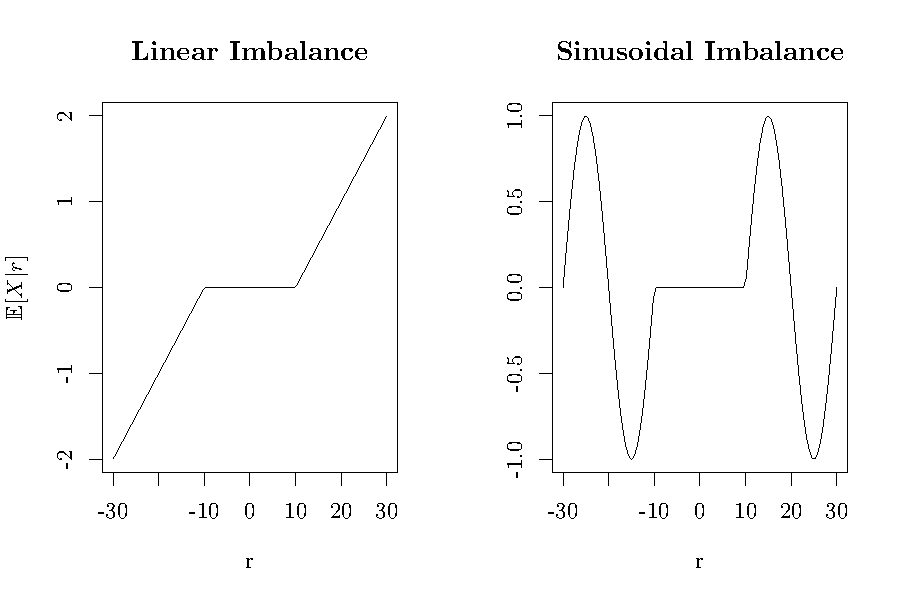
\includegraphics[width=\maxwidth]{figure/illlustrateSim-1} 

\caption{Two designs for the simulation study.}
\label{fig:illustrateSim}
\end{figure}

In each dataset, the researcher tests $H_d$, $d=1,...,30$ via t-tests
and records the p-values.
These p-values, in turn, give rise to eight different choices for
$\hat{d}$: $\dalphaU$ and $\dalphaB$, with $\alpha=0.5,0.15,0.25$,
$\dhatm$, and $\dhatmab$.

Figure \ref{fig:linImb} shows the results of 1000 replications
under linear imbalance.
Table \ref{tab:linear} shows some statistics that may not be apparent
from the figure.
For all three sample sizes, the model selectors tended to select
samples that were too large.
However, as the sample size increased, and with it the power to reject
$H_b$ for smaller values of $b$, the performance of the selectors
improved.
$\dalphaU$ had the smallest
variance across the board, but at the
price of often choosing the larger datasets.
On the other extreme, $\dalphaB$ picked very small datasets---for all
three sample sizes, $\dhatB_{0.25}\le 3$ in over half of the
simulation runs.

$\dhatm$ and $\dhatmab$, on average, performed the best across
runs---their average choices were close to $\dstar=10$ in all three
runs.
However, they were more variable than $\dalphaU$, and occasionally
chose very small $\hat{d}$.
The flexible estimate $\dhatmab$ was less than or equal to $\dhatm$ in
every case, though the two estimates coincided about
70\% of the time.



\begin{figure}

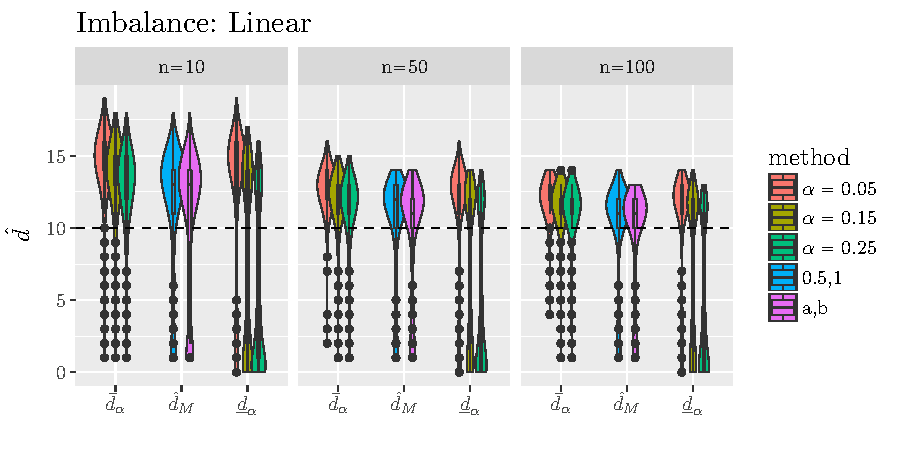
\includegraphics[width=\maxwidth]{figure/linearImbalance-1} 

\caption{Simulation results for simulations featuring linear
  imbalance. The parameter $n$ controls the sample size at each value
  of $r$, from -30 to 30. Eight different model selectors are shown
  for each sample size via overlaid violin and box-plots}
\label{fig:linImb}
\end{figure}


% latex table generated in R 3.3.1 by xtable 1.8-2 package
% Wed Feb  8 18:46:10 2017
\begin{table}[ht]
\centering
\begin{tabular}{r|cccc|cccc|cccc|}
  & \multicolumn{4}{c}{$n=10$}&\multicolumn{4}{c}{$n=50$} &\multicolumn{4}{c}{$n=100$}\\
 \hline
 & avg & sd & $\le 3$ & $>13$ & avg & sd & $\le 3$ & $>13$ & avg & sd & $\le 3$ & $>13$ \\ 
  \hline
$\dhatU_{0.05}$ & 14.7 & 2.2 & 0.01 & 0.79 & 12.7 & 1.4 & 0.00 & 0.26 & 12.1 & 1.1 & 0.00 & 0.04 \\ 
  $\dhatU_{0.15}$ & 13.5 & 2.7 & 0.02 & 0.60 & 12.0 & 1.9 & 0.01 & 0.12 & 11.5 & 1.7 & 0.01 & 0.02 \\ 
  $\dhatU_{0.25}$ & 12.8 & 2.9 & 0.02 & 0.47 & 11.5 & 2.2 & 0.02 & 0.07 & 11.1 & 2.0 & 0.02 & 0.01 \\ 
  $\dhatB_{0.05}$ & 12.3 & 5.2 & 0.14 & 0.65 & 10.9 & 4.2 & 0.13 & 0.20 & 10.3 & 4.0 & 0.14 & 0.02 \\ 
  $\dhatB_{0.15}$ & 8.1 & 6.0 & 0.36 & 0.29 & 7.6 & 5.2 & 0.34 & 0.03 & 7.2 & 5.1 & 0.36 & 0.00 \\ 
  $\dhatB_{0.25}$ & 5.7 & 5.6 & 0.52 & 0.14 & 5.3 & 5.1 & 0.52 & 0.00 & 5.1 & 4.9 & 0.52 & 0.00 \\ 
  $\dhatm$ & 11.7 & 4.3 & 0.10 & 0.43 & 10.4 & 3.6 & 0.10 & 0.05 & 10.0 & 3.5 & 0.12 & 0.00 \\ 
  $\dhatmab$ & 10.8 & 4.7 & 0.14 & 0.34 & 9.8 & 4.0 & 0.15 & 0.03 & 9.4 & 3.8 & 0.15 & 0.00 \\ 
   \hline
\end{tabular}
\caption{The average and standard deviation of each selection rule $\hat{d}$, as well as the proportions of runs each method selected $d\le 3$ or $d>13$, for $n=10,50,100$ with linear covariate imbalance} 
\label{tab:linear}
\end{table}


When departures from $H_d$ are not monotonic in $d$, as in the
sinusoidal simulation, differences between model selectors can be
starker.
Figure \ref{fig:sinImb} shows the results from that simulation.
Most striking is that $\dalphaU$ chooses the maximum $d=30$ rather
frequently.
This may not actually be a bad thing---indeed, the mean of the
covariate $X$ is equal between positive and negative $r$ when $d=30$.
However, depending on the application, large differences in the mean
of $X$ for particular values of $r$ may indicate other departures from
model assumptions.
Whether the behavior exhibited by $\dalphaU$, which occasionally
chooses the largest possible $d$, is preferable to that of $\dhatm$,
which rarely does, will depend on the specific data scenario.
That said, the results in Figure \ref{fig:sinImb} illustrate the
difference between a procedure like $\dalphaU$ whose decision may be driven by one
individual p-value, and one like $\dhatm$ which is driven by the
entire distribution of p-values.


\begin{figure}

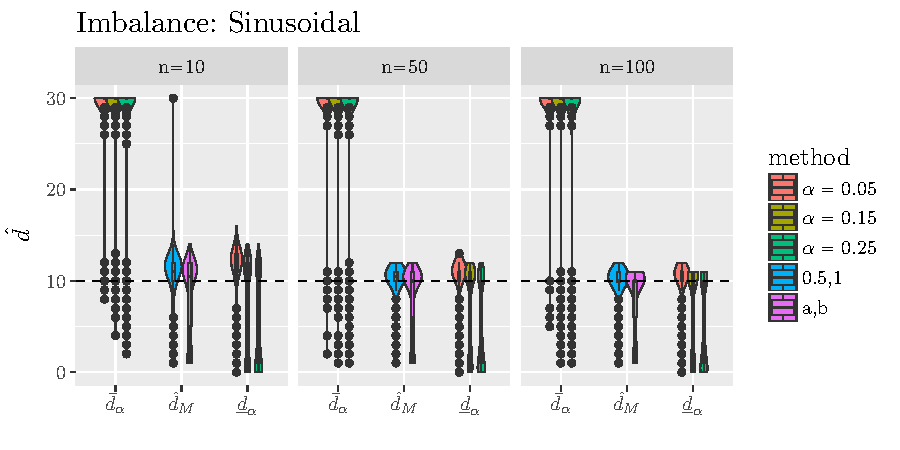
\includegraphics[width=\maxwidth]{figure/sinusoidalImbalance-1} 

\caption{Simulation results for simulations featuring sinusoidal
  imbalance. The parameter $n$ controls the sample size at each value
  of $r$, from -30 to 30. Eight different model selectors are shown
  for each sample size via overlaid violin and box-plots}
\label{fig:sinImb}
\end{figure}




\section{Two Data Examples}\label{sec:examples}

This section will present a more complete treatment of the two
examples from Section \ref{sec:exampleIntro}: choosing a bandwidth in
a regression discontinuity design, and choosing a lag order for an
autoregressive model.
The two examples correspond to two broad categories of
specification: selecting data to analyze and
selecting a model specification.

\subsection{SSTs in Regression Discontinuity Bandwidth Selection:
  Estimating the Effect of  Academic Probation on College GPAs}

At many universities, students who fail to achieve a minimum GPA are
put on academic probation (AP) \citep[See, e.g.][]{tovar2006academic}.
This provides them access to a set of resources designed to address
personal issues that may be hindering their  performance.
Perhaps more importantly, AP is a threat---students on AP who do not
improve are subject to disciplinary measures such as suspension.
\citet{lso} recognized that AP can form a regression discontinuity
design (RDD), in which treatment is a function of a ``running
variable'' with a pre-determined cutoff.
Specifically the treatment $Z$, students' AP status, is (almost) a
deterministic function of a ``running variable'' $R$, students'
grade-point-averages (GPAs).
Students with a GPA below a pre-determined cutoff, $R<c$, are put on AP.
That being the case, students with GPAs just below $c$ may be
comparable to students with GPAs just above $c$---comparing these two
sets of students allows researchers to estimate the effect of AP on
outcomes $Y$.
The challenge becomes defining ``just above'' and ``just below''; SSTs
may be able to play a role here.

For example, \citet*{cft} (CFT) suggests directly
comparing the outcomes of subjects with $R$ very close to $c$, say with
$R\in [c-bw,c+bw]$ for some bandwidth $bw>0$
To choose $bw$, CFT uses pre-treatment covariates $\bm{X}$, and
covariate balance tests range of candidate bandwidths.
For each possible $bw$, they test the hypothesis that the covariates
are balanced:
\begin{equation}\label{eq:covBal}
\bm{X}\independent Z| R\in[c-bw,c+bw]
\end{equation}
and choose the largest bandwidth in which (\ref{eq:covBal}) cannot be
rejected.

Bandwidth selection for RDDs, and the role of covariate balance tests,
encompasses a growing literature.
As its name suggests, regression discontinuity typically relies on
regression modeling: the goal is to model $Y$ as a function of $R$ on
either side of $c$ to estimate the average treatment effect for
subjects with $R$ in an infinitesimally-small interval around the
cutoff $c$ \citep[See][]{imbensLemiuxRDD}.
In contrast, CFT dispenses with regression altogether.
One popular way to ensure robustness to model misspecification is to
fit the regression models to a subset of the data with $R$ in a
window around $c$.
A number of methods exist to choose an optimal bandwidth $bw$---the width
of the window---that is both large enough to allow for precise effect
estimation but small enough to ensure robustness.
\citet{IK} suggest using non-parametric estimates of the curvature of
the regression function of $Y$ on $R$, combined with local linear
regression, to choose a $bw$ that minimizes mean-squared-error.
However, other authors have suggested choosing $bw$ (or an analogous quantity) based on
SSTs, including \citet{mattai}, which presents a Bayesian approach
analogous to CFT's, \citet{salesHansen}, which discusses the use of robust
regression models,  and \citet{angristWanna}, which proposes a method
to estimate effects for subjects with $R$ farther from $c$.
In the latter paper, SSTs do not test covariate balance, but the
irrelevance of $R$ conditional on covariates $X$, for subjects in a
given bandwidth.

This section will illustrate several approaches to SSTs in the context
of estimating the effect of AP for first year college students on
subsequent GPAs.
For the sake of simplicity, the discussion will be limited to CFT's
general approach to regression discontinuity designs; however, many of
the SST methods can be extended to other RDD analyses.
In their analysis, \citet{lso}  considered a set of seven covariates:
students' high-school GPA (expressed in percentiles), age at college
matriculation, number of attempted credits, gender, native language
(English or other), birth place (North America or other) and
university campus (the university consisted of three campuses).
A version of Hotellings $T^2$ test that models
treatment assignment $Z$, and not $X$, as random \citep{hansenBowers}
is used to test balance.
The resulting p-values are plotted in the left panel of Figure \ref{fig:rdpvalues1}.
Various bandwidth selections are plotted as vertical lines in the
figure, and enumerated in Table \ref{tab:RDD}.

\begin{figure}
\begin{knitrout}
\definecolor{shadecolor}{rgb}{0.969, 0.969, 0.969}\color{fgcolor}
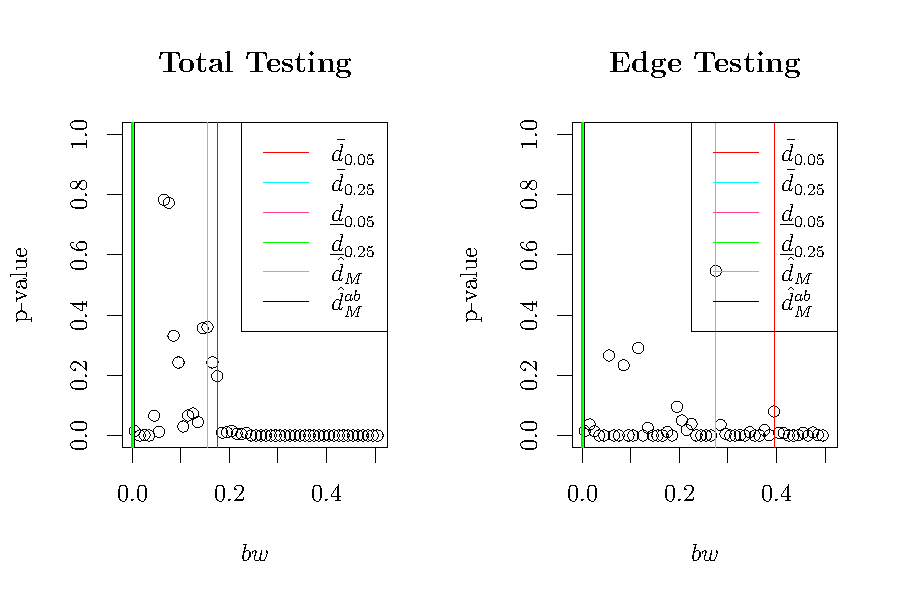
\includegraphics[width=\maxwidth]{figure/rdd-1} 

\end{knitrout}
\caption{P-values from for balance in all seven covariates
  from the \citet{lso} analysis and only high school GPA, respectively. Vertical lines denote bandwidth choices using
  different criteria.}
\label{fig:rdpvalues1}
\end{figure}

% latex table generated in R 3.3.1 by xtable 1.8-2 package
% Wed Feb  8 18:46:34 2017
\begin{table}[ht]
\centering
\begin{tabular}{r|ccc|ccc|}
  & \multicolumn{2}{c}{All Covariates}&\multicolumn{2}{c}{HS GPA}\\
 \hline
 & d & bw & ATE & d & bw & ATE \\ 
  \hline
$\bar{d}_{0.05}$ & 18 & 0.175 & 0.11 (0.028) & 18 & 0.175 & 0.11 (0.028) \\ 
  $\bar{d}_{0.15}$ & 18 & 0.175 & 0.11 (0.028) & 16 & 0.155 & 0.13 (0.03) \\ 
  $\underline{d}_{0.05}$ & 0 & N/A & NA (NA) & 18 & 0.175 & 0.11 (0.028) \\ 
  $\underline{d}_{0.15}$ & 0 & N/A & NA (NA) & 1 & 0.005 & 0.22 (0.122) \\ 
  $\dhatm$ & 1 & 0.005 & 0.22 (0.122) & 16 & 0.155 & 0.13 (0.03) \\ 
  $\dhatmab$ & 1 & 0.005 & 0.22 (0.122) & 16 & 0.155 & 0.13 (0.03) \\ 
   \hline
\end{tabular}
\caption{Selected RDD bandwidths---'d' is the point in the sequence selected, and 'bw' is the bandwidth---using covariate balance tests for all the covariates in \citet{lso} and only high school GPA, respectively, along with their assosicated estimates for the average treatment effect of academic probation (ATE), with standard errors.} 
\label{tab:RDD}
\end{table}


The p-values from testing balance on all covariates do not follow a
monotonic pattern---they are near zero for very small bandwidths,
larger for bandwidths greater than 0.035, and close to zero again for
bandwidths greater than 0.175.
Here, as in the sinusoidal simulation in Section \ref{sec:simulation},
social scientists may disagree about appropriate bandwidth selection.
On the one hand, covariates appear to be approximately balanced (or,
at least, there is no evidence to the contrary) for a range of
bandwidths.
On the other hand, the apparent covariate imbalance for small
bandwidths is worrying: perhaps it suggests deeper problems with this
design---suggesting either using regression to adjust for trends in
the running variable, or abandoning the design altogether.

This ambivalence is reflected in the various bandwidth selectors.
$\dhatB_{0.05}$ and $\dhatB_{0.15}$ reject every possible bandwidth, while
both $\dhatm$ and $\dhat_M^{a,b}$ select the lowest possible
bandwidth of 0.
According to these methods, the CFT method is unsuitable for this
dataset.
However, the scattered large p-values at some bandwidths lead
 $\dalphaU$ to select larger bandwidths.

To better illustrate differences between the window selection
strategies, we consider the covariate high school GPA alone.
Since the outcome of interest is itself a GPA, prior measures of GPA
are arguably the most relevant and important to control.
P-values from tests of balance in high school GPA are
displayed in the right panel of Figure \ref{fig:rdpvalues1}.
Fortunately for the illustration here, high school GPA may be
balanced for small bandwidths.
These p-values from are more nearly
monotonic, appearing roughly uniformly distributed for smaller
bandwidths and close to zero at high bandwidths.
The behavior of bandwidth selectors $\dhat$, shown with vertical lines
in the figure and in Table \ref{tab:RDD}, reflects this feature.
The first p-value below 0.05 occurs at a bandwidth of
0.185; accordingly, both $\dhatU_{0.05}$ and
$\dhatB_{0.05}$ select a bandwidth of 0.175.
On the other hand, the p-value of 0.0704 at 0.015
caused $\dhatB_{0.15}$ to select the smallest possible bandwidth of 0.
The change-point selectors, $\dhatm$ and $\dhatmab$, along with
$\dhatU_{0.15}$, chose a bandwidth of 0.155.
In fact, a close inspection of Figure \ref{fig:rdpvalues1} reveals
that beginning at a bandwidth of 0.1, the p-values seem to be
decreasing---suggesting, perhaps, slight violations of the assumption
in (\ref{eq:covBal}).
$\dhatm$ and $\dhatmab$ chose a higher bandwidth than this due, in
part, to the high p-value at 0.15, which broke the trend, but
otherwise may have chosen an even smaller bandwidth.
In contradistinction, selectors such as $\dalphaU$ and $\dalphaB$ that
are based entirely on individual extreme p-values cannot account for
such patterns.

Table \ref{tab:RDD} also gives the estimated average treatment effect
for each bandwidth.
At very small bandwidths, the estimated effect is larger, though with a
large standard error as well.
The choice between bandwidths at the higher end does not make a large
difference in the estimated effects.

\subsection{Lag Order in AR($p$) Models: US Total Unemployment}


Figure \ref{fig:example}B shows the natural logarithm of the United States total
unemployment rate from 1890 to 2016.
The data were combined from the ``Nelson \& Plosser extended data
set'' provided in the \texttt{urca} library in \texttt{R}
\citep{urca,Rcite}, which covers years 1890--1988, and a downloadable
dataset from the United States Bureau of Labor Statistics, itself
derived from the Current Population Survey, which covers years
1947--2015 \citep{cps}.
The two datasets agree on the overlapping years.

Assume that the time series follows an ``AR($d$)'' model; that is,
\begin{equation}\label{eq:arp}
unemp_t=\mu + \displaystyle\sum_{i=1}^d \phi_i unemp_{t-i}+\epsilon_t
\end{equation}
where $\mu$ and $\{\phi_i\}_{i=1}^d$ are parameters to be estimated
and $\epsilon_t$ is white noise.
In this model, the unemployment in one year is a function of
unemployment rates in the previous $d$ years, but conditionally
independent of even earlier measurements.
More generally, we may write (\ref{eq:arp}) as
\begin{equation}\label{eq:arpinf}
unemp_t=\mu+\displaystyle\sum_{i=1}^\infty \phi_i
unemp_{t-i}+\epsilon_t
\end{equation}
with $\phi_i=0$ for $i>d$.

Having settled on model (\ref{eq:arp}), the analyst must choose $d$,
the lag order.
SSTs can be useful here \citep[e.g.][]{practitionersGuide}.
Consider the null hypothesis $H_d: \phi_i=0$ for all $i>d$;
a researcher could test a sequence of such null hypotheses, for a set
of plausible values of $d$, and choose the $d$ based on the results.
Of course, there are other options for choosing $d$, including
substantive theory or optimizing
information criteria, like AIC or BIC
(\citep{akaike1969fitting,schwarz1978estimating} though
\citealt{potscher1991effects} points out that differences in AIC or
BIC are essentially likelihood ratio test statistics).
In the absence of substantive theory, SSTs can assist a modeler to
choose the smallest model that is still approximately correct---as
opposed to the model that maximizes predictive accuracy as measured
by, say, mean squared error.
A large literature surrounds this important question \citep[See,
e.g.][and the citations
therein]{mcquarrie1998regression,liew2004lag}. This section is not
meant as a complete treatment, or even an overview, of lag order
selection, but as an illustration of SSTs in a well-known area.

Figure \ref{fig:tspvalues1} gives the p-values from a sequence
likelihood ratio tests, as described in \citet[][Ch.1]{urca}, which
discussed a similar dataset.
For each candidate lag order $d$, the likelihood ratio test compares
twice the ratio of the log likelihoods of $AR(d+1)$ and $AR(d)$ models
to a $\chi^2_1$ distribution.
If the $AR(d+1)$ model fits much better than the $AR(d)$ model, a lag
order of $d$ may not be sufficient.
The p-values follow a stark pattern: for $d<5$, they are close to
zero, while for $d\ge5$, they appear roughly uniformly distributed.

Table \ref{tab:ts}, and vertical lines in Figure \ref{fig:tspvalues1},
show the lag order choices from $\dalphaU$, $\dalphaB$, $\dhatm$, and
$\dhatmab$, which are based on the p-values, and the lag orders that
minimize AIC and BIC, based directly on the models' likelihood and numbers
of parameters.
Here, smaller models are preferable to larger models, so $\dstar$ is
the \emph{smallest} acceptable value for $d$.
This is the opposite of the RDD case, which attempted to find the
\emph{largest} dataset on which to fit the model.






The change-point selectors $\dhatm$ and $\dhatmab$ both selected a
lag order of 5, consistent with the casual
observation that p-values for lags less than this value are very
small, while those greater appear approximately uniform.
Incidentally, the two information criteria considered, AIC and BIC,
agreed with this choice, as did $\dhatU_{0.15}$.
In contradistinction, $\dhatU_{0.05}$ chose a smaller lag order of
3, since the corresponding p-value of
0.066 slightly exceeds the threshold of 0.05.

At the other extreme, the $\dalphaB$ selectors both chose very large
models with $d=$17, due to the presence of
of a small p-value of
0.044 at
$d=$16.

This example illustrates how considering the entire distribution of
p-values, as $\dhatm$ does, can lead to better model selection than
considering only the small (as in $\dalphaB$) or large ($\dalphaU$)
values.

\begin{figure}

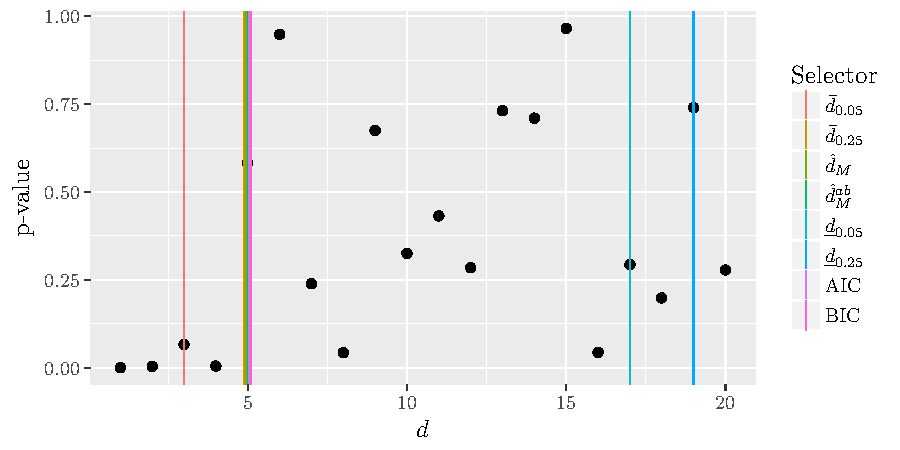
\includegraphics[width=\maxwidth]{figure/tsResults-1} 

\caption{P-values from sequential likelihood-ratio tests of model fit,
  comparing models AR($d$) with AR($p+1$)o in the annual total US
  unemployment rate (logged) time series.}
\label{fig:tspvalues1}
\end{figure}


% latex table generated in R 3.3.1 by xtable 1.8-2 package
% Thu Feb  9 00:06:59 2017
\begin{table}[ht]
\centering
\begin{tabular}{rr}
  \hline
 & Lag Order \\ 
  \hline
$\bar{d}_{0.05}$ &   3 \\ 
  $\bar{d}_{0.25}$ &   5 \\ 
  $\underline{d}_{0.05}$ &  17 \\ 
  $\underline{d}_{0.25}$ &  19 \\ 
  $\dhatm$ &   5 \\ 
  $\dhatmab$ &   5 \\ 
  AIC &   5 \\ 
  BIC &   5 \\ 
   \hline
\end{tabular}
\caption{Lag order selections for an $AR(d)$ model of the US unemployment time series.} 
\label{tab:ts}
\end{table}


\section{Discussion}\label{sec:discussion}
The simple intuition behind the use of SSTs is that there exists a set
of candidate models that are approximately correct, and another set
that are false.
By examining the results of specification tests, the thinking goes, a
researcher may pick the best model from the former category.
However, the negative logic of specification tests makes them poorly
suited to finding the boundary between the two groups.
Further, they require the choice of a tuning parameter---the level
$\alpha$---and there is little guidance as to how to choose it.
Finally, common procedures for choosing a model based on a sequence of
hypothesis tests are driven entirely by individual extreme test
results, and may, therefore, be unstable.

This paper argues that a clever idea from the change point literature
can solve all of these problems.
\citet{mallik} suggests that the full distribution of p-values from
SSTs may be used to construct an estimator of the optimal true model
in the sequence.
The estimator they suggest does not require researchers to specify
$\alpha$ and is not typically driven by individual extreme p-values.
Just as \citet{hodgeslehmann} showed how to estimate a parameter from
a sequence of p-values from hypothesis tests, \citet{mallik} shows how
to select an optimal model from a sequence of p-values from
specification tests.

This paper examined the performance of the selector from
\citet{mallik} and other SST-based selectors via simulation and
example, and showed that, in certain ways, it tends to perform better,
if only marginally so.
In the simulation studies, its average value was consistently closer
to the correct value than the other methods.
It successfully compromised between the two dominant strategies,
denoted here as $\dalphaU$ and $\dalphaB$, typically avoiding the
over-aggressiveness of $\dalphaU$ while also avoiding the
occasionally extreme conservativeness of $\dalphaB$.
Its advantage came from its ability to overlook intermittent anomalous
p-values that distract $\dalphaU$ or $\dalphaB$ from an overall
pattern.

There are several open questions regarding $\dhatm$'s behavior and
use.
First, it is unclear whether or when the more flexible version
$\dhatmab$ should be preferred to $\dhatm$---there is good reason to
expect it to perform better when sample sizes are small, but is there
a cost associated with using $\dhatmab$ in larger samples?

Further, there may be ways to construct SSTs in a way that improves
$\dhatm$'s performance.
For instance, tests that focus on the difference between two
successive models, as opposed to each model's overall quality, may, in
some circumstances, have higher power to detect departures from
assumptions.
Such tests would yield p-values with less statistical dependence,
which would provide another advantage to $\dhatm$.
How to construct such tests, and under what circumstances, if any,
they improve model selection, is a topic for future research.

Researchers who want to use hypothesis tests to choose from a sequence
of models may feel uneasy about the statistical validity of their
procedure or their choice of $\alpha$.
This paper will hopefully show how to choose a model using a sequence
of p-values in a way that is coherent and does not require arbitrary
cutoffs or tuning parameters.



\bibliographystyle{plainnat}
\bibliography{sst}


\end{document}
